\ifCLASSOPTIONcompsoc
  \IEEEraisesectionheading{\section{Introduction}}
\else
  \section{Introduction}
\fi
  \IEEEPARstart{T}{he} computational demands for image pattern recognition have risen substantially over the past decade, driven largely by the success of Convolutional Neural Networks (CNNs) in 2D image processing. In response, several hardware accelerator architectures have been developed. Hardware acceleration has proven successful for both 2D~\cite{mittal2020survey} and 3D~\cite{mittal2021survey} CNN implementations.

  A variety of optimization approaches have been developed for the task of accelerating CNNs, including: efficient memory access~\cite{han2016cnn,jiang2021optimized,doumet2024h2pipe}, parallelization methods~\cite{jouppi2020domain,choquette2021nvidia} often via systolic-array inference~\cite{chua2022systolic}, optimizing floating-point operations~\cite{fan2021high}, quantizing weights and activations~\cite{finotti2021quant,he2023research,salah2025post}, and addressing data sparsity~\cite{jiang2021optimized,fan2021high}.

  Complementing hardware acceleration, another strategy involves the creation of more efficient convolution algorithms. The standard discrete convolution algorithm, as well as the more widely used matrix-multiplication (MMX), have a base asymptotic complexity of $O(N^2)$, scaling very poorly with image and kernel sizes. This is particularly relevant for 3D CNNs, as the computational load of their convolutional layers can rapidly dominate that of all other layers combined~\cite{hegde2018morph}.

  In 2016, Lavin \& Gray~\cite{lavin2016fast} reviewed the relevant convolution algorithms --- which were, at the time, MMX and FFT convolution --- and proposed a new class of algorithms based on the Coppersmith–Winograd series of matrix multiplication methods~\cite{coppersmith1982asymptotic}. Further development of convolution algorithms with improved asymptotic complexity~\cite{karstadt2020matrix,schwartz2023pebbling} presents a critical trade-off: the theoretical gain in efficiency is often offset by the computational overhead and implementation complexity of the required transforms, limiting their practical utility. Consequently, the Winograd class of convolution algorithms has become the de facto standard for hardware-efficient CNN designs~\cite{shen2018towards,barabasz2019winograd,vardhana2025high}.

  The computational advantages of FFT-based convolution are negated in modern CNN architectures for two primary reasons. First, its efficiency is contingent upon large kernel sizes~\cite{lavin2016fast}, which have been largely superseded by the prevalent use of small, 3x3 kernels in deeper networks~\cite{simonyan2014very}. Second, its inherent reliance on Complex-domain operations presents a significant implementation barrier for high-level design methodologies.
  
  Subsequent research has produced optimizations for FFT convolution, including methods like convolution splitting~\cite{chitsaz2020acceleration}, overlap-add~\cite{highlander2016very,chen2024fast}, and mixed-radix FFT~\cite{meng2024high}. These advances, along with the development of spectral CNNs~\cite{pratt2017fcnn,liu2021accelerating,ayat2019spectral,han2021deep,watanabe2021image}, have renewed its relevance for architectures that inherently employ large kernels, such as 3D CNNs~\cite{nguyen2016energy, lan2017high, li20243d}.

  Despite these advances, the high operational complexity of Complex multiplication is still a burden. Current FPGA-based solutions employ parallelization~\cite{li2024split} and pipelining~\cite{fan2021high} to mitigate latency. However, these strategies leverage increased hardware resources to mask the high operation count rather than reducing it. Consequently, the underlying hardware efficiency (measured as throughput per component) remains unimproved.

  It is possible to reduce the operation count of Complex multiplication by representing its inputs as polar coordinates~\cite{lera2023hardware}. This was first implemented for CNNs in 2024 by Reis \textit{et al.}~\cite{reis2024phasor} using high-level synthesis (HLS) and achieving promising results. While an important tool for quickly implementing designs, HLS CNN applications have been frequently criticized regarding resource underutilization~\cite{xu2024flare,jiang2025fpga,antunes2025fpga}, high power consumption~\cite{salman2020comparative} and general performance issues~\cite{faber2022challenges,ahmed2023autohls,lau2024rapidstream}. This is opposed to RTL models, written in hardware-description languages (HDL), where low-level optimizations are available at the cost of longer development cycles.

  \ifCLASSOPTIONcompsoc\else % this needs to be at second column of the first page
    \IEEEpubidadjcol
  \fi
  
  We propose an FFT-based 3D-convolution accelerator using hardware-efficient polar-coordinate multiplication, an FFT pipeline, and optimized for large images using input slicing and overlap-add. We synthesize the architecture using HDL and implement it in a VC709 FPGA board. By validating our implementation using state-of-the-art benchmarks, we demonstrate the viability of FFT convolution in non-spectral 3D CNNs.
  
  This document is organized as follows: in Section~\ref{sec:alg} we discuss the state-of-the-art convolution algorithms and their computational complexity; in Section~\ref{sec:imp} we describe the design choices, optimizations, and testing procedures of our proposed architecture; Section~\ref{sec:res} lists the results obtained and comparisons to the state-of-the-art; Section~\ref{sec:rela} discusses related work; and Section~\ref{sec:conc} presents our conclusions.

  \ifCLASSOPTIONcompsoc
    \begin{figure*}[!tb]\centering
  \else
    \begin{figure*}[!t]\centering
  \fi
    \subfloat[]{%
      \makebox[0.9\columnwidth]{%
        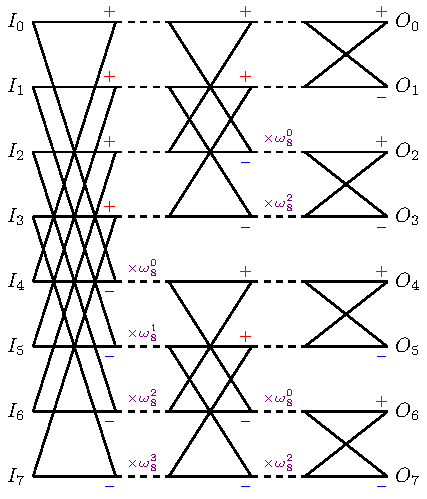
\includegraphics{fig/fft-1.pdf}\label{fig:fft1}}}\qquad%
    \subfloat[]{%
      \makebox[0.9\columnwidth]{%
        
\includegraphics{fig/fft-0.pdf}\label{fig:fft2}}}%
    \caption{Visual representation of an 8-point radix-2 FFT using decimation in frequency (a) and decimation in time (b).}\label{fig:fft}
  \end{figure*}

\section{Convolution Algorithms}\label{sec:alg}
  Lavin \& Gray~\cite{lavin2016fast}, as well as later publications~\cite{shen2018towards}, have performed comparative algorithmic analyses of MMX, Winograd, and FFT convolution. We will add to their analyses by addressing the scalability of these algorithms and how this property affects the total complexity of the system.

  The nomenclature used henceforth, which is based on previous works in the field~\cite{lavin2016fast,shen2018towards,fan2021high}, is defined as such:
  %
  \begin{itemize}
    \item $I$ is a 3D input channel with dimensions $\{I_x,I_y,I_z\}$. There are $I_c$ input channels. Each of its elements are defined as $I[ix, iy, iz, c]$.
    \item $K$ is a 3D convolution kernel with dimensions $\{K_x,K_y,K_z\}$. There are $K_f$ kernels, being $K[kx, ky, kz, f]$.
    \item $I[c]*K[f]$ is the convolution of one channel $I$ and one kernel $K$. There are $I_c$ output channels and $K_c$ filter maps.
  \end{itemize}

  The output dimensions are a function of the respective sizes of $I$ and $K$ and depend on the \textit{mode} of convolution, as follows:
  %
  \begin{itemize}
    \item \textit{Full:} $O_d = I_d + K_d - 1$
    \item \textit{Same:} $O_d = I_d$
    \item \textit{Valid:} $O_d = I_d - K_d$
  \end{itemize}
  
  The baseline method of discrete convolution used by CNNs uses \textit{Same} mode and can be defined as:
  %
  \begin{equation}
    \begin{gathered}
      I[c]*K[f] = \\\sum_{z=0}^{K_z}\sum_{y=0}^{K_y}\sum_{x=0}^{K_x}I[ox+kx,oy+ky,oz+kz,c]K[x,y,z,f].
    \end{gathered}
  \end{equation}

  This method shares its complexity with the commonly used matrix-multiplication algorithm~\cite{lera2023hardware}. To simplify calculations, we consider the total number of multiplications required by each algorithm: $M$. For discrete and matrix-multiplication convolutions, this number is equal to the product of each dimension processed:
  %
  \begin{equation}\label{eq:MM-mul}
    \begin{gathered}
      M = I_xI_yI_zI_cK_xK_yK_zK_f.
    \end{gathered}
  \end{equation}

  \subsection{FFT convolution}
    Lower complexity can be achieved via the Convolution Theorem:
    %
    \begin{equation}
      I[c] * K[f] = \mathcal{F}^{-1}(\mathcal{F}(I[c]) \cdot \mathcal{F}(K[f])),
    \end{equation}
    %
    where $\cdot$ represents the pointwise product (also known as \textit{Hadamard} product), and $\mathcal{F}$ and $\mathcal{F}^{-1}$ represent the Discrete Fourier Transform (DFT) and its inverse (IDFT). This method produces a \textit{full} mode convolution.

    The class of algorithms known as \textit{Fast Fourier Transforms} (FFT) are used to compute the DFTs. By definition, an FFT computes an $N$-point DFT in $O(N\log_2N)$. The standard radix-2 FFT~\cite{gauss1866nachlass,cooley1965algorithm} breaks down the DFT into $\log_2N$ steps, each consisting of multiple ``butterfly operations'' paired with twiddle-factor multiplications. The order of operations depends on the recursion method used: Decimation in Frequency (DIF) or Decimation in Time (DIT), as illustrated by Figures~\ref{fig:fft1} and \ref{fig:fft2}, respectively. Each ``butterfly'' receives a pair $(A,B)$ and outputs $(A+B,A-B)$, where $A$ and $B$ are Complex numbers. Each twiddle factor multiplier calculates a product by a root-of-unity $\omega$ with the form:
    %
    \begin{equation}
      \omega_{N}^{k} = e^{\frac{2{\pi}i}{N}k},
    \end{equation}
    %
    where $k \in \mathbb{Z} \cap [0,N-1]$.
    
    While the input signal of the FFT is one-dimensional, it is possible to represent an arbitrary number of dimensions using zero-padding. Figure~\ref{fig:Ma} represents a 2x2x2 signal $K$. To convolve this array with another signal of the same shape, we first pad each dimension $d$ by $2d-1$, thus conveying its dimensionality and avoiding cyclic convolution. Figure~\ref{fig:Mb} represents the padded signal; the gray line displays the order of rasterization.

    \ifCLASSOPTIONcompsoc
      \begin{figure*}[!tb]\centering
    \else
      \begin{figure*}[!t]\centering
    \fi
      \subfloat[]{%
        \makebox[0.7\columnwidth]{%
          
\includegraphics{fig/matrix-0.pdf}\label{fig:Ma}}}\qquad%
      \subfloat[]{%
        \makebox[0.9\columnwidth]{%
          
\includegraphics{fig/matrix-1.pdf}\label{fig:Mb}}}%
      \caption{A three-dimensional signal (a) and the required zero-padding to avoid cyclic convolution (b).}\label{fig:M}
    \end{figure*}

    The rasterized signal is further padded to its next power of two, so that radix-2 FFT can be applied across $\log_2N$ stages. The size of the resulting array, denoted $N$, as a function of the sizes of $K$, is:
    %
    \begin{equation}\label{eq:N}
      N = 2^{\ceil{\log_2(2K_x-1){\times}\log_2(2K_y-1){\times}\log_2(2K_z-1)}}.
    \end{equation}

    The transformed array produced by the FFT chain is subject to \textit{hermitian symmetry}. Assume an $N$-point array of Complex numbers $(a+bi)$. The array has hermitian symmetry if each point with index $[N/2+1]$ to $[N-1]$ is equivalent to the Complex conjugate $(a-bi)$ of the points with index $[N/2-1]$ to $[1]$, respectively. This means that almost half of the array is redundant and can be inferred by switching the sign bit of its y-component. This property is preserved after the pointwise multiplication, so the total number of pointwise Complex multiplications required by FFT convolution is:
    %
    \begin{equation}
      M(\mathbb{C}) = \frac{N}{2}+1.
    \end{equation}

    In order to convolve $I$ and $K$ using FFT, the sizes of each transformed array must be equal. Direct zero-padding of the kernel to match the input dimensions is computationally inefficient for CNNs, as the significant size disparity ($I \gg K$) increases the cost of the subsequent transform. Instead, we can ``slice'' the input into kernel-sized pieces and convolve each slice with the kernel. The overlapping points of each convolution are added together, forming the complete output. This is known as \textit{overlap-add}~\cite{smith1997scientist,chen2024fast} and is a form of algorithmic scaling.

    Let $S$ be a 3D slice of $I$ over $K$, with dimensions $\{K_x,K_y,K_z\}$. The number of slices on each dimension is $\{S_x,S_y,S_z\}$, such that:
    %
    \begin{equation}
      S_{x} = \left\lceil\frac{I_x}{K_x}\right\rceil;\quad
      S_{y} = \left\lceil\frac{I_y}{K_y}\right\rceil;\quad
      S_{z} = \left\lceil\frac{I_z}{K_z}\right\rceil.
    \end{equation}

    A Complex-domain multiplication can be performed with 4 Real-domain multiplications. Let $X$ and $Y$ be Complex numbers such that $X=a+bi$ and $Y=c+di$. The product of the two signals is:
    %
    \begin{equation}\label{eq:cmul-rect}
      XY = (a+bi)(c+di) = (ac-bd) + (ad+bc)i.
    \end{equation}

    Using this method, the total number of multiplications required by FFT convolution is:
    %
    \begin{equation}\label{eq:fconv-mul1}
      M = 
      4
      \left\lceil\frac{I_x}{K_x}\right\rceil
      \left\lceil\frac{I_y}{K_y}\right\rceil
      \left\lceil\frac{I_z}{K_z}\right\rceil
      \left(\frac{N}{2}+1\right).
    \end{equation}

    However, $X$ and $Y$ can also be represented in polar coordinates such that $X=A\phase{\alpha_1}$ and $Y=B\phase{\alpha_2}$, where $A,B$ are radial distances and $\alpha_1,\alpha_2$ are angular coordinates:
    %  
    \begin{equation}\label{eq:cmul-pol}
      XY = A\phase{\alpha_1} \cdot B\phase{\alpha_2} = AB\phase{\alpha_1+\alpha_2}.
    \end{equation}

    This representation reduces the total operation count to 1 Real multiplication and 1 Real addition. Section~\ref{sec:imp} describes the algorithm used to implement the conversions between these coordinate systems. Notably, these conversions do not incur any multiplications, and as such:
    %
    \begin{equation}\label{eq:fconv-mul2}
      M = 
      \left\lceil\frac{I_x}{K_x}\right\rceil
      \left\lceil\frac{I_y}{K_y}\right\rceil
      \left\lceil\frac{I_z}{K_z}\right\rceil
      \left(\frac{N}{2}+1\right).
    \end{equation}

  \subsection{Winograd}
    Similarly to FFT convolution, the Winograd method transforms the input and kernel into a domain (more strictly, a \textit{field}) where pointwise multiplication is equivalent to the convolution of the original signals~\cite{lavin2016fast}. In three dimensions, the algorithm defines convolution as $F(m^3,r^3)$, where $m$ and $r$ are integers. Let $A$ and $B$ be matrices that contain $I[c]$ and $K[f]$ such that their total size is equal to $(m+r-1)^3$ and $r^3$, respectively. Convolution is then expressed as:
    %
    \begin{equation*}
      A * B  = (Z( (XAX^T)^RX^T \cdot (YAY^T)^RY^T )Z^T)^RZ^T,
    \end{equation*}
    %
    where $X$, $Y$, and $Z$ are transform matrices, the superscript $R$ denotes clockwise rotation, and $T$ denotes transposing. The result of this operation has size $m^3$ and produces a \textit{valid} mode convolution.

    The transform matrices depend on $m$, $r$, and the point-selection procedure used. 3D CNN applications require at least $F(2^3,3^3)$ and trivial matrices for this operation have been found, such as the set used by Shen \textit{et al.} (2018)~\cite{shen2018towards}:
    %
    \begin{equation*}
      \begin{gathered}
        X = 
        \begin{bmatrix}
          1 &  0 & -1 &  0\\
          0 &  1 &  1 &  0\\
          0 & -1 &  1 &  0\\
          0 &  1 &  0 & -1
        \end{bmatrix},\quad
        Y = 
        \begin{bmatrix}
          1 & 0 & 0\\
          \frac{1}{2} & \frac{1}{2} & \frac{1}{2}\\
          \frac{1}{2} & -\frac{1}{2} & \frac{1}{2}\\
          0 & 0 & 1
        \end{bmatrix},\\\rule{0pt}{6ex}
        Z = 
        \begin{bmatrix}
          1 &  1 &  1 &  0\\
          0 &  1 & -1 & -1
        \end{bmatrix}.
      \end{gathered}
    \end{equation*}

    These transform matrices do not incur any multiplications, as multiplying by $\frac{1}{2}$ can be computed as a right-bit-shift. Higher values of $m$ and $r$ incur different matrices where this property cannot be guaranteed.

    It is possible to calculate multiple $F(m^3,r^3)$ convolutions and add the overlapping points to form a complete output~\cite{lan2017high}. However, this approach differs from the FFT method in that it requires calculating one convolution per stride of the kernel, as the output is \textit{valid} type. For an image $I$ and stride 1, the total number of multiplications is:
    %
    \begin{equation}\label{eq:wino-mul}
      \left\lceil\frac{I_x-r}{m}\right\rceil
      \left\lceil\frac{I_y-r}{m}\right\rceil
      \left\lceil\frac{I_z-r}{m}\right\rceil
      (m+r-1)^3.
    \end{equation}

  \subsection{Comparison}
    Figures \ref{fig:alg1} and \ref{fig:alg2} are plots of Equations \ref{eq:MM-mul} (baseline), \ref{eq:wino-mul} (Winograd), \ref{eq:fconv-mul1} (FFT convolution), and \ref{eq:fconv-mul2} (FFT convolution using polar multiplication), for different kernel sizes and assuming $K$ is equilateral and has size $k$. Figure~\ref{fig:alg1} assumes $I=(k+1)^3$, or one semi-convolution. Figure~\ref{fig:alg2} assumes $I=128{\times}171{\times}16$, the input size used by C3D~\cite{tran2015learning}, a 3D CNN widely used as a benchmark.

    \ifCLASSOPTIONcompsoc
      \begin{figure*}[!tb]\centering
    \else
      \begin{figure*}[!t]\centering
    \fi
      \subfloat[]{%
        \makebox[0.95\columnwidth]{%
          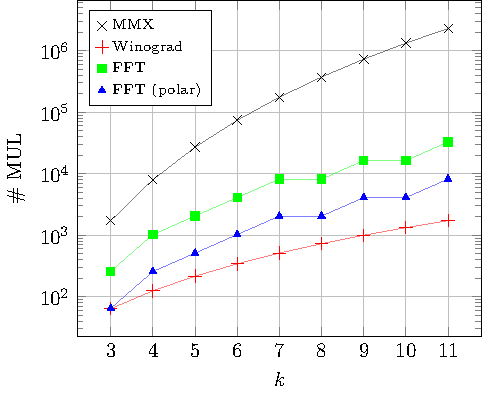
\includegraphics{fig/plot-0.pdf}\label{fig:alg1}}}\qquad%
      \subfloat[]{%
        \makebox[0.95\columnwidth]{%
          
\includegraphics{fig/plot-1.pdf}\label{fig:alg2}}}%
      \caption{Number of multiplications (log scale) vs kernel-size for $I=4{\times}4{\times}4$ (a) and $I=128{\times}171{\times}16$ (b).}\label{fig:alg}
    \end{figure*}

    These graphs do not account for the multiplications stemming from Winograd's transform at higher kernel-sizes, nor the twiddle-factor multiplications used by FFT convolution, as both of them are multiplications by constants and are optimized at synthesis time.

\section{Implementation}\label{sec:imp}
  In order to convert the image and kernel between rectangular and polar coordinates, we implement CORDIC ({\bf{CO}}ordinate {\bf{R}}otation {\bf{DI}}gital {\bf{C}}omputer)~\cite{volder1959cordic}, a trigonometric algorithm that iteratively calculates the rotation of a given vector by decreasingly-sized angles. It has two modes of operation: rotation and vectorization; as well as three inputs, here labeled $(x,y,z)$. 

  When configured for vectorization, the CORDIC algorithm iteratively transforms the rectangular coordinates from $(x_0,y_0)$ into radial distance and angular coordinates $(x_j,y_j)$ after $j$ iterations. In the complementary rotation mode, CORDIC transforms a Complex number $(x_0,z_0)$ from polar to rectangular $(x_j,y_j)$ coordinates after $j$ iterations. This is generally expressed as:
  %
  \begin{equation}\label{eq:cordic1}
    \begin{bmatrix}
      x_{j+1} \\
      y_{j+1} \\
      z_{j+1}
    \end{bmatrix}
    =
    \begin{bmatrix}
      x_{j} - \sigma_{j}2^{-j}y_{j} \\
      y_{j} + \sigma_{j}2^{-j}x_{j} \\
      z_{j} + \sigma_{j}\arctan(2^{-j})
    \end{bmatrix},
  \end{equation}
  %
  where
  %
  \begin{equation}\label{eq:cordic2}
    \sigma_j = 
    \begin{cases}
      sign(y_j),~\text{in}~\textbf{vectorization}~\text{mode} \\
      -sign(z_j),~\text{in}~\textbf{rotation}~\text{mode}
    \end{cases}.
  \end{equation}

  The precision of the algorithm is equivalent to $2^{-j}$, or one bit of precision per iteration. Note that when using fixed-point notation, it is sufficient to iterate once for each bit after the point. We denote the total number of bits of a variable as $S_t$ and the number of bits after the point as $S_p$. Our implementation defaults to 24 and 16, respectively.

  A simple hardware implementation of CORDIC consists of two $S_t$-bit adders, one $S_p$-bit adder, two variable bit-shifters, three registers, and a lookup table for storing $\arctan(2^{-j})$.
  
  The outputs of $x_j$ and $y_j$ are scaled (as a consequence of CORDIC's inner algorithm) by a constant $\kappa_j$ on each iteration, where:
  %
  \begin{equation}\label{eq:cordic3}
    \kappa_j = \cos(\arctan(2^{-j})),
  \end{equation}
  %
  and must be corrected to obtain the desired result. The correction can be made after the process completes, by multiplying each output by the scaling factor:
  %
  \begin{equation}\label{eq:cordic4}
    \frac{1}{\kappa} = \prod_{j=0}^{S_p-1}{\frac{1}{\sqrt{1+2^{-2j}}}} \stackrel{S_p=16}{\approx} 0.60725.
  \end{equation}

  % BCA: depois de step, referenciar a equacao
  In the pointwise multiplication step (\ref{eq:cmul-pol}), CORDIC is used 3 times. The first two convert the image slice and kernel to polar coordinates and the last converts the result back to rectangular coordinates. The scaling factor carries over across operations, including pointwise multiplication, and as such we can apply the correction at any point in the process (image, kernel, or product). The combined scaling factor is:
  %
  \begin{equation}\label{eq:cordic5}
    \frac{1}{\kappa^3} \stackrel{S_p=16}{\approx} 0.22393.
  \end{equation}

  Complex multiplication in polar coordinates involves the addition of phase angles. This sum can exceed the $[-\pi, \pi]$ boundary where CORDIC is defined, introducing a phase-wrapping ambiguity. To circumvent this, we store the \textit{quadrant} of each angular coordinate in the unit circle, normalize them to the first quadrant, perform the add operation, and convert the result into its appropriate quadrant. To simplify this computation, we divide each $\arctan(2^{-j})$ by $2\pi$. The resulting binary, encoded in 16-bits, represents fractions of $\pi$, with its two most-significant bits representing the quadrant of the vector in the unit circle, as shown in Figure~\ref{fig:pfb}. This allows quick access to the quadrant of the angle, as well as enabling normalization to any quadrant by simply setting its first two bits.

  \ifCLASSOPTIONcompsoc
    \begin{figure}[!tb]\centering
  \else
    \begin{figure}[!t]\centering
  \fi
    
\includegraphics[width=0.9\columnwidth]{fig/unit_circle-0.pdf}
    \caption{Four symmetric angles encoded as $\pi$-fractions.}\label{fig:pfb}
  \end{figure}
  
  CORDIC's complexity does not increase with the image- or kernel-sizes, depending instead on $S_p$ which gives it a relative asymptotic complexity of $O(1)$ and enables a trade-off between numerical precision and arithmetic complexity.

  To avoid dedicated Complex multipliers, a common technique is to employ the CORDIC algorithm for twiddle-factor rotations in the FFT pipeline~\cite{banerjee2001fpga,choudhary2011cordic}. Each CORDIC iteration rotates the input by elementary angles which coincide with the twiddle-factors used by the FFT. However, this process applies the gain factor $\kappa$ to all points that weren't multiplied by a twiddle-factor. The consequent scale correction increases the implementation cost in LUT resources. Considering this trade-off, we opted to implement the twiddle-factor rotations using DSP blocks, balancing the DSP and LUT costs.

  Our twiddle-factor multiplication design using DSPs is a variant of the Karatsuba multiplication algorithm~\cite{karatsuba1962multiplication}. Using the previously established nomenclature for Complex numbers, Karatsuba defines three intermediate variables:
  %
  \begin{equation}\label{eq:kara1}
    \begin{cases}
      k_1 = c {\times} (a+b) \\
      k_2 = b {\times} (c+d) \\
      k_3 = a {\times} (d-c)
    \end{cases},
  \end{equation}
  %
  such that
  %
  \begin{equation}\label{eq:kara2}
    XY = (k_1 - k_2) + (k_1 + k_3)i.
  \end{equation}

  The direct implementation of this algorithm requires 5 additions and 3 multiplications. However, for twiddle-factor multiplication, the values $c$ and $d$ are constant. Consequently, $(c+d)$ and $(d-c)$ are also constant and can be precomputed and stored, reducing the operational cost to 3 additions and 3 multiplications. This represents a substantial improvement over the standard Complex multiplication (\ref{eq:cmul-rect}) which requires 2 additions and 4 multiplications.
  
  \subsection{Pipelining}\label{ssec:pipe}
    To achieve high throughput, the proposed design employs a fully-pipelined architecture, detailed in Figure~\ref{fig:pipeline}. The pipeline is organized into two phases, separated by the dashed boundary. This organization enables the reuse of hardware components across phase boundaries, an optimization that enhances hardware efficiency by reducing resource utilization compared to a replicated design.

    \ifCLASSOPTIONcompsoc
      \begin{figure*}[!tb]\centering
    \else
      \begin{figure*}[!t]\centering
    \fi
      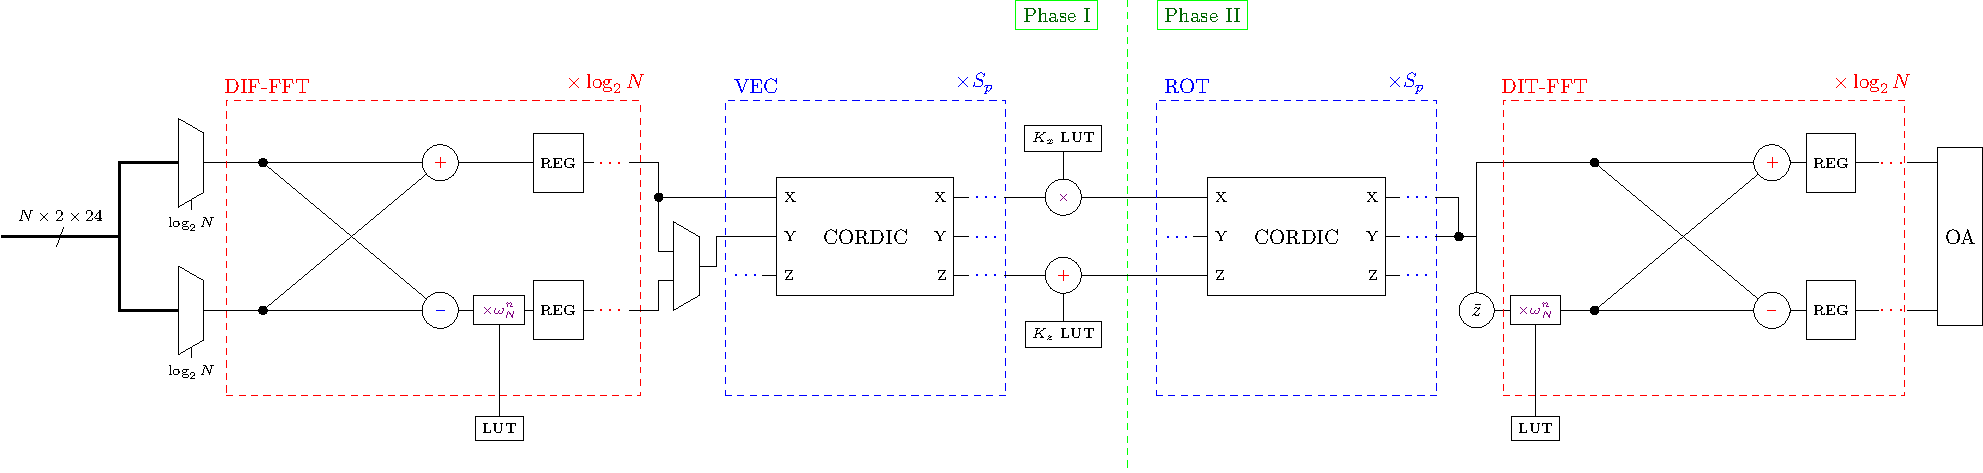
\includegraphics[width=2.04\columnwidth]{fig/pipeline-0.pdf}
      \caption{Fully-pipelined FFT convolution design using overlap-add and CORDIC.}\label{fig:pipeline}
    \end{figure*}

    In Phase-I, the system rasterizes and pads the 3D slice as shown in Figure~\ref{fig:M}, then multiplexes it into the FFT chain.

    The FFT is divided into $\log_2N$ stages, where $N$ is defined by Equation~\ref{eq:N}. Each stage consists of one butterfly, one twiddle-factor multiplication block, and a set of registers. The data entering the first FFT stage is still on the Real domain. As such, we arranged this FFT in DIF mode (see figure \ref{fig:fft1}), as this mode places most non-redundant twiddle-factor multiplications at the first stage, significantly simplifying these operations.
    
    The add and subtract blocks within the butterflies are (on every layer except the first) Complex operation blocks, and as such constitute two operations each. We implemented the twiddle-factor multiplication blocks (past the first stage) using Karatsuba, resulting in 3 adders and 3 multipliers each, along with a lookup table that is shared across stages. Many of these operations will be optimized away by the synthesizer, as about half the input array are zeroes. Some twiddle factors are also trivial to multiply, such as $\omega^{0}=1$ and $\omega^{\frac{N}{4}}=i$.

    Each FFT node processes two input points per machine cycle and stores the result into the register bank. On the next cycle, the node processes two more points, the next stage reads the result, and the process repeats along the chain. Once the pipeline is full, the FFT chain is capable of processing two input points per cycle.

    Hermitian symmetry carries over through CORDIC and polar multiplication. As such, the points past $N/2$ can be inferred later. The edge case for index $N/2$ still needs to be calculated, as it is not the Complex conjugate of index $0$. Its insertion into the next block is done via a multiplexer.

    The CORDIC chain is set to vectorization on Phase-I to perform the conversion to polar coordinates. There are $S_p$ CORDIC blocks which, when fully pipelined, process two points (one symmetrical) of the original array.

    In Phase-I, each slice $S$ of each channel $I_c$ is processed up to the conversion to polar coordinates and is stored in a register bank. After the process is complete, Phase-II begins, where each slice is multiplied by each kernel $K_f$. In this phase, the CORDIC chain is set to rotation mode and the FFT is rearranged into DIT mode. This process is managed by a control unit and routing elements, not depicted in the diagram to avoid cluttering.

    The polar multiplication step consists of one multiplier and one adder, in accordance to Equation~\ref{eq:cmul-pol}. The kernels are processed at synthesis time and their Complex polar coordinates are stored in their respective lookup tables. Before being stored, each kernel's radial distance is multiplied by $\kappa$ (see Equation~\ref{eq:cordic5}), which applies the correction to each point of the array without inferring additional multiplier blocks.

    The output of CORDIC during Phase-II is joined at the final stage, forming one point of the $N$-sized array. The respective Complex conjugate (denoted $\bar{z}$) is inferred and sent into the FFT chain. The $N/2$ exception to hermitian symmetry is always a Real number whose polar-coordinate conversion is trivial and need not be processed by CORDIC.
    
    The FFT chain then executes the inverse transform. The last stage of DIF is equivalent to the first stage of DIT (see Figure~\ref{fig:fft}), allowing data to flow seemingly along the pipeline. As the mirror to DIF, DIT places most non-redundant twiddle-factor multiplications at the end. The data leaving the pipeline is on the Real domain, as all Complex components shall cancel-out.

    Finally, the overlap-add module (OA) receives the two Real points and adds them to the respective indexes in the feature map. This process is repeated for all channels and all kernels. Consequently, Phase-II is $K_f$ times longer than Phase-I, and for large $K_f$ (as is usual for modern CNNs), Phase-II is responsible for nearly all processing time.

  \subsection{Parallelism}
    The design in Figure~\ref{fig:pipeline} is compact and scalable, useful for implementation across a range of FPGA devices. However, we can further improve the hardware efficiency of the design using parallelism.

    Previously, we synthesized one butterfly and twiddle-factor multiplier per FFT stage. We can instead synthesize every block on each stage, allowing the synthesizer to better optimize the redundant twiddle-factor multiplications.

    To maintain uninterrupted data flow along the pipeline, we scale the CORDIC chain accordingly. Similarly to the FFT chain, many CORDIC blocks will become redundant and will be optimized away during synthesis. We also parallelize the polar multiplication and overlap-add stages, which now complete one slice per cycle in Phase-II.

    We label this version of the architecture \textbf{parallel-core}, while the design described in Section~\ref{ssec:pipe} is accordingly labeled \textbf{pipelined-core}.
    
\subsection{Synthesis \& Testing}\label{ssec:synth}
  We synthesized and implemented both designs on a VC709 FPGA board. The system achieved timing closure at 150 MHz for parallel-core and 200 MHz for pipelined-core, due to routing and congestion factors. Table~\ref{tab:ru} displays the resource usage metrics of both cores for $K = 3{\times}3{\times}3$. 

  The functional correctness and numerical precision of the design were verified against a golden reference model implemented in C/C++. The validation methodology consisted of two phases: extensive randomized testing, where outputs were compared iteratively to a double-precision floating-point convolution, and targeted edge-case analysis using inputs with extreme values to evaluate boundary conditions (large and small inputs).

  \ifCLASSOPTIONcompsoc
    \begin{table}[!tb]
  \else
    \begin{table}[!t]
  \fi
    \caption{Resource usage of pipelined and parallel cores in VC709 environment.}
    \centering
    \label{tab:ru}
    \begin{tabular}{|c|c|c|c|}\hline
      Core       & DSP    & LUT    & FF     \\\hline
      Pipelined  & 1      & 5861   & 4265   \\\cline{2-4}
      [usage]    & 0.03\% & 1.3\%  & 0.5\%  \\\hline
      Parallel   & 65     & 296572 & 213376 \\\cline{2-4}
      [usage]    & 1.8\%  & 66.9\% & 25.6\% \\\hline
    \end{tabular}
  \end{table}

  \ifCLASSOPTIONcompsoc
    \begin{table*}[!tb]
  \else
    \begin{table*}[!t]
  \fi
    \caption{Comparison of different FPGA accelerator architectures applied on C3D.}
    \centering
    \label{tab:he-comp}
    \begin{tabular}{|c|c|c|c|c|c|c|}
      \hline
      Project &
        \multicolumn{2}{c|}{Shen \textit{et al.} (2018)~\cite{shen2018towards}} &
        Liu \textit{et al.} (2019)~\cite{liu2019uniform} &
        Fan \textit{et al.} (2021)~\cite{fan2021high} &
        Yang \textit{et al.} (2023)~\cite{yang2023fgpa} &
        Our Design\\\hline
      Algorithm    & \multicolumn{2}{c|}{Winograd} & MMX      & MMX         & MMX    & FFT    \\\hline
      Precision    & \multicolumn{2}{c|}{16-fixed} & 16-fixed & $<$16-float & (unmentioned)   & 16-fixed \\\hline
      Board                       & VC709 & VUS440 & VC709    & GX1150      & XCZU15 & VC709  \\\hline
      Technology (nm)             & 28    & 20     & 28       & 20          & 16     & 28     \\\hline
      Frequency (MHz)             & 150   & 200    & 120      & 220         & 100    & 150    \\\hline
      DSP                         & 1536  & 1536   & 3595     & 1345        & 1317   & 65     \\\hline
      Throughput ($GOP/s$)        & 474.3 & 940.6  & 667.7    & 1536        & 209.4  & 107.8  \\\hline
      Resource efficiency (\ref{eq:mu-he})
        &                           0.31  & 0.61   & 0.19     & 1.14        & 0.16   & 1.66   \\
      Normalized (\ref{eq:mu-nhe})
        &                           2.06  & 3.06   & 1.55     & 5.19        & 1.59   & 11.05  \\\hline
    \end{tabular}
  \end{table*}

  Throughput ($GOP/s$) was measured using the first convolutional layer of C3D~\cite{tran2015learning}, where $I=128{\times}171{\times}3$, $I_c=3$, and $K_f=16$. Resource efficiency was measured as the product of throughput and number of DSPs inferred~\cite{fan2021high,li2022hardware,kyriakos2022resources,jiang2025fpga}. We express this as:
  %
  \begin{equation}\label{eq:mu-he}
    \frac{GOP}{s{\times}DSP}.
  \end{equation}

  This metric can be normalized across different FPGA devices by dividing it by the operational frequency~\cite{meyer2020evaluating, montgomerie2023pass, jiang2025fpga}. We express this as:
  %
  \begin{equation}\label{eq:mu-nhe}
    \frac{GOP}{s{\times}DSP{\times}MHz}.
  \end{equation}

\section{Results}\label{sec:res}
  Our fixed-point implementation, using a software 24-bit format with 16 fractional bits, achieved a worst-case error of $2^{-8}$ across all hardware validation tests. This error bound ensures correctness in the 16 most significant bits and falls within the known tolerance for low-precision CNN operations, making it suitable for both training and inference tasks~\cite{courbariaux2014training}.

  To the extent of our research regarding FPGA-based acceleration of 3D CNNs, Fan \textit{et al.} (2021)~\cite{fan2021high} achieves the highest resource efficiency. Their choice of convolution algorithm is the standard matrix-multiplication except using floating-point quantization to achieve efficient operations. Shen \textit{et al.} (2018)~\cite{shen2018towards} remains the most resource-efficient FPGA-based accelerator that uses Winograd convolution and is capable of processing 3D convolutional filters.

  Table~\ref{tab:he-comp} displays the throughput ($GOP/s$), hardware efficiency (\ref{eq:mu-he}), and normalized hardware efficiency (\ref{eq:mu-nhe}) of our parallel-core design and the state-of-the-art. This comparison is analogous to the ones made by previous projects in their analyses~\cite{shen2018towards,fan2021high}. Liu \textit{et al.}~\cite{liu2019uniform} and Yang \textit{et al.}~\cite{yang2023fgpa} have also contributed to the state-of-the-art and were included in this comparison.

\section{Related Work}\label{sec:rela}
  CNN acceleration is a broad and actively-researched field. This section covers some relevant bibliography not previously cited.
  
  Software-based network architectures and hardware accelerators can be used in tandem to achieve higher performance and efficiency. Spectral CNNs~\cite{pratt2017fcnn,liu2021accelerating,ayat2019spectral,han2021deep,watanabe2021image} as well as rotation-invariant CNNs~\cite{kim2020cycnn,mo2024ric} avoid the need to transform between the Real and Complex domains when using FFTs. This incurs changes across each layer of the network, and more research is needed to evaluate whether the impacts on accuracy and development cycles are worth the performance gain.

  Since Shen \textit{et al.} (2018)~\cite{shen2018towards}, algorithmic optimizations of the Winograd method have been published~\cite{barabasz2019winograd,barabasz2020error,alam2022winograd} but have not yet been implemented in an FPGA-based accelerator. There exist more recent applications of the algorithm for CNNs~\cite{kala2019high,jiang2025fpga}, but they are not trivially expandable to three dimensions.

  Winograd and FFT convolutions may be able to benefit from similar quantization methods as the ones used by Fan \textit{et al.}~\cite{fan2021high}. Their implementation does not optimize the total number of operations of the algorithm, instead optimizing the operations themselves, leaving room for algorithmic optimizations.
  
  The possibility of designing CNNs using CORDIC-based activation functions has been proposed~\cite{shen2024efficient, kokane2025retrospective}. This would likely lead to more optimal accelerators using FFT convolution.

  There exist other FFT algorithms, such as split-radix~\cite{sorensen2003computing} and prime-factor~\cite{burrus1981place} FFTs, which might be useful in optimizing slice dimensions.

\section{Conclusions \& Future Work}\label{sec:conc}
  This work has established the lower computational complexity of FFT convolution using the overlap-add method and introduced a corresponding FPGA accelerator that leverages polar-coordinate multiplication to achieve state-of-the-art resource efficiency. 
  
  The primary resource cost in our design is attributed to the twiddle-factor multiplications within the FFT pipeline, pointing to a clear target for future work. Potential for improvement includes the algorithmic optimizations discussed in Section~\ref{sec:rela} and implementation on more advanced FPGA architectures. 
  
  The results presented herein strongly indicate that FFT convolution, when combined with overlap-add and an optimized polar multiplication unit, represents the most efficient approach for accelerating 3D CNNs and other architectures that depend on large-kernel operations.